\documentclass[11pt]{article}
\usepackage[a4paper, margin=1in]{geometry}
\usepackage{amsfonts,amsmath,amssymb,mathtools}
\usepackage[none]{hyphenat}
\usepackage{fancyhdr}
\usepackage{graphicx}
\usepackage[parfill]{parskip} %Removes indentation on new paragraph 
\usepackage{tkz-euclide}

\pagestyle{fancy}
\fancyhead{} %clears default header
\fancyfoot{} %clears default footer
\fancyhead[L]{Ethan Lim} %\slshape makes itallics

\begin{document}

\section*{Question 5}
The in-center of a triangle is the point equidistant from the triangles
sides.
% , and we take for granted the fact that the in-center can be equivalently defined
% as the point where the three angle bisectors of the triangle intersect.

\begin{center}
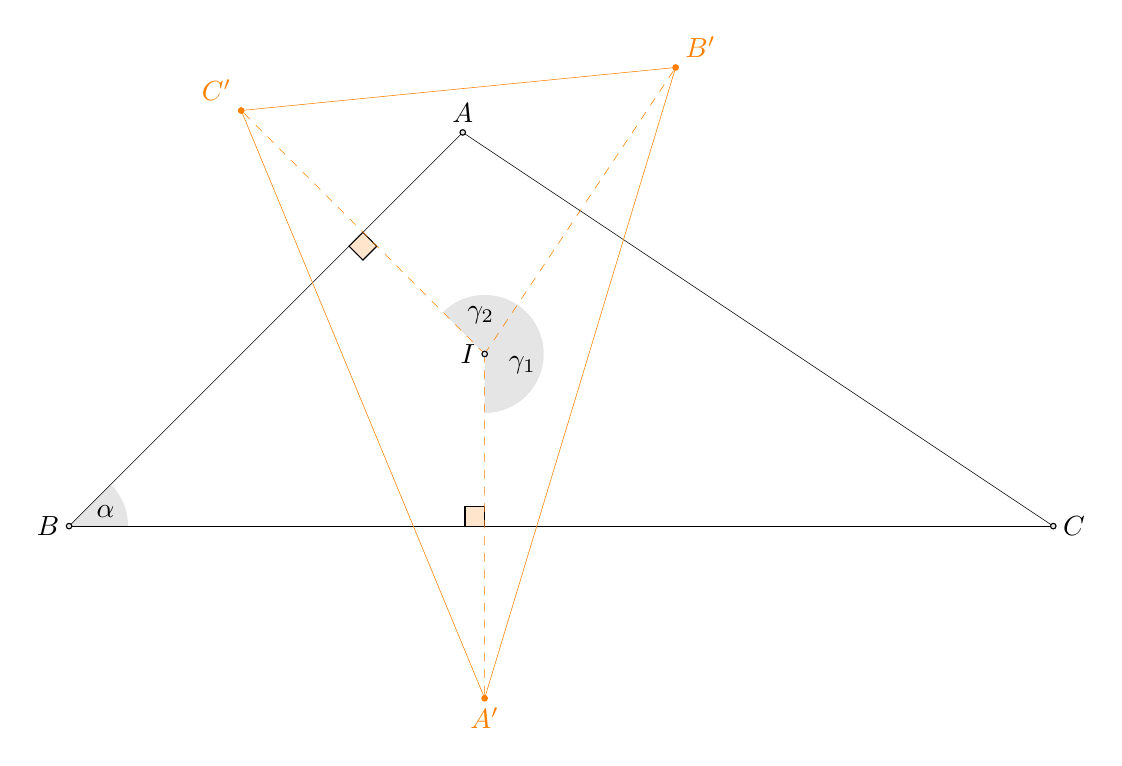
\begin{tikzpicture}[scale=2.5]
	% initial points
	\tkzDefPoint(2,2){A}
	\tkzDefPoint(0,0){B}
	\tkzDefPoint(5,0){C}

	% incenter
	\tkzDefTriangleCenter[in](A,B,C)
	\tkzGetPoint{I}

	% reflected points
	\tkzDefPointBy[reflection=over B--C](I)
	\tkzGetPoint{A'}
	\tkzDefPointBy[reflection=over A--C](I)
	\tkzGetPoint{B'}
	\tkzDefPointBy[reflection=over A--B](I)
	\tkzGetPoint{C'}

	% mark right angles
	\tkzInterLL(A,B)(I,C')
	\tkzGetPoint{d}
	\tkzInterLL(B,C)(I,A')
	\tkzGetPoint{e}
	
	\tkzMarkRightAngle[fill=orange!20,size=0.1](B,d,I)
	\tkzMarkRightAngle[fill=orange!20,size=0.1](B,e,I)

	% angles
	\tkzFillAngle[size=0.3,fill=gray!20](C,B,A)
	\tkzFillAngle[size=0.3,fill=gray!20](A',I,B')
	\tkzFillAngle[size=0.3,fill=gray!20](B',I,C')

	\tkzLabelAngle[pos=0.2](C,B,A){$\alpha$}
	\tkzLabelAngle[pos=0.2](A',I,B'){$\gamma_1$}
	\tkzLabelAngle[pos=0.2](B',I,C'){$\gamma_2$}

	% draw lines
	\tkzDrawSegment(A,B)
	\tkzDrawSegment(B,C)
	\tkzDrawSegment(C,A)

	\tkzDrawSegment[orange,dashed](I,A')
	\tkzDrawSegment[orange,dashed](I,B')
	\tkzDrawSegment[orange,dashed](I,C')

	% draw points
	\tkzDrawPoints(A,B,C,I)
	\tkzDrawPoints[orange](A',B',C')
	\tkzDrawSegment[orange](A',B')
	\tkzDrawSegment[orange](B',C')
	\tkzDrawSegment[orange](C',A')

	% label points
	\tkzLabelPoint[above](A){$A$}
	\tkzLabelPoint[left](B){$B$}
	\tkzLabelPoint[right](C){$C$}
	\tkzLabelPoint[left](I){$I$}
	\tkzLabelPoint[color=orange,below](A'){$A'$}
	\tkzLabelPoint[color=orange,above right](B'){$B'$}
	\tkzLabelPoint[color=orange,above left](C'){$C'$}

\end{tikzpicture}
\end{center}

Let $\alpha=\angle ABC$

\end{document}